% Graphic for TeX using PGF
% Title: /mnt/hgfs/patrick/middleware/paper/scheme-chunks.dia
% Creator: Dia v0.97.2
% CreationDate: Sat Aug 17 22:09:48 2013
% For: patrick
% \usepackage{tikz}
% The following commands are not supported in PSTricks at present
% We define them conditionally, so when they are implemented,
% this pgf file will use them.
\ifx\du\undefined
  \newlength{\du}
\fi
\setlength{\du}{15\unitlength}
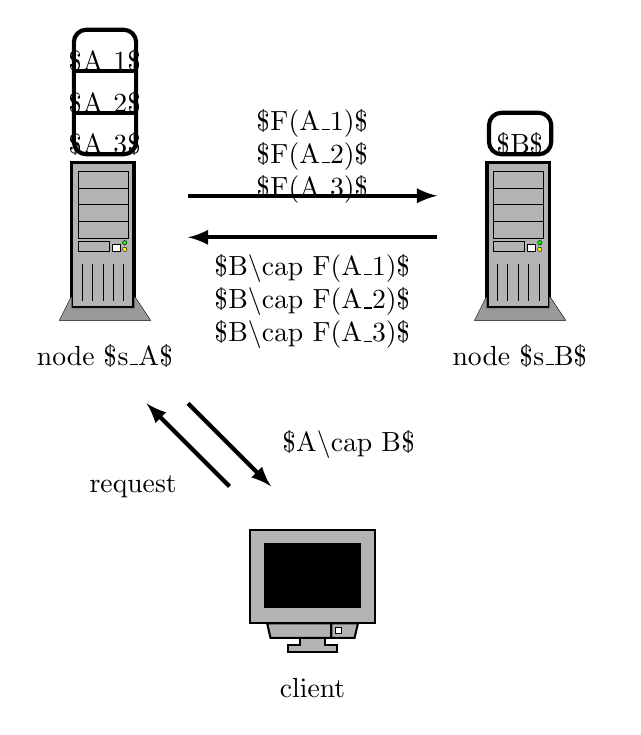
\begin{tikzpicture}
\pgftransformxscale{1.000000}
\pgftransformyscale{-1.000000}
\definecolor{dialinecolor}{rgb}{0.000000, 0.000000, 0.000000}
\pgfsetstrokecolor{dialinecolor}
\definecolor{dialinecolor}{rgb}{1.000000, 1.000000, 1.000000}
\pgfsetfillcolor{dialinecolor}
\pgfsetlinewidth{0.100000\du}
\pgfsetdash{}{0pt}
\pgfsetdash{}{0pt}
\pgfsetbuttcap
{
\definecolor{dialinecolor}{rgb}{0.000000, 0.000000, 0.000000}
\pgfsetfillcolor{dialinecolor}
% was here!!!
\definecolor{dialinecolor}{rgb}{0.000000, 0.000000, 0.000000}
\pgfsetstrokecolor{dialinecolor}
\draw (6.250000\du,2.000000\du)--(7.750000\du,2.000000\du);
}
\pgfsetlinewidth{0.100000\du}
\pgfsetdash{}{0pt}
\pgfsetdash{}{0pt}
\pgfsetbuttcap
{
\definecolor{dialinecolor}{rgb}{0.000000, 0.000000, 0.000000}
\pgfsetfillcolor{dialinecolor}
% was here!!!
\definecolor{dialinecolor}{rgb}{0.000000, 0.000000, 0.000000}
\pgfsetstrokecolor{dialinecolor}
\draw (6.250000\du,1.000000\du)--(7.750000\du,1.000000\du);
}
\pgfsetlinewidth{0.100000\du}
\pgfsetdash{}{0pt}
\pgfsetdash{}{0pt}
\pgfsetroundjoin
{\pgfsetcornersarced{\pgfpoint{0.300000\du}{0.300000\du}}\definecolor{dialinecolor}{rgb}{0.000000, 0.000000, 0.000000}
\pgfsetstrokecolor{dialinecolor}
\draw (6.250000\du,0.000000\du)--(6.250000\du,3.000000\du)--(7.750000\du,3.000000\du)--(7.750000\du,0.000000\du)--cycle;
}\pgfsetlinewidth{0.100000\du}
\pgfsetdash{}{0pt}
\pgfsetdash{}{0pt}
\pgfsetroundjoin
{\pgfsetcornersarced{\pgfpoint{0.300000\du}{0.300000\du}}\definecolor{dialinecolor}{rgb}{0.000000, 0.000000, 0.000000}
\pgfsetstrokecolor{dialinecolor}
\draw (16.250000\du,2.000000\du)--(16.250000\du,3.000000\du)--(17.750000\du,3.000000\du)--(17.750000\du,2.000000\du)--cycle;
}\pgfsetlinewidth{0.100000\du}
\pgfsetdash{}{0pt}
\pgfsetdash{}{0pt}
\pgfsetbuttcap
\pgfsetmiterjoin
\pgfsetlinewidth{0.080000\du}
\pgfsetbuttcap
\pgfsetmiterjoin
\pgfsetdash{}{0pt}
\definecolor{dialinecolor}{rgb}{0.701961, 0.701961, 0.701961}
\pgfsetfillcolor{dialinecolor}
\fill (6.200000\du,3.200000\du)--(6.200000\du,6.700000\du)--(7.700000\du,6.700000\du)--(7.700000\du,3.200000\du)--cycle;
\definecolor{dialinecolor}{rgb}{0.000000, 0.000000, 0.000000}
\pgfsetstrokecolor{dialinecolor}
\draw (6.200000\du,3.200000\du)--(6.200000\du,6.700000\du)--(7.700000\du,6.700000\du)--(7.700000\du,3.200000\du)--cycle;
\pgfsetlinewidth{0.010000\du}
\pgfsetbuttcap
\pgfsetmiterjoin
\pgfsetdash{}{0pt}
\definecolor{dialinecolor}{rgb}{0.000000, 0.000000, 0.000000}
\pgfsetstrokecolor{dialinecolor}
\draw (6.350000\du,3.410000\du)--(6.350000\du,3.810000\du)--(7.550000\du,3.810000\du)--(7.550000\du,3.410000\du)--cycle;
\pgfsetbuttcap
\pgfsetmiterjoin
\pgfsetdash{}{0pt}
\definecolor{dialinecolor}{rgb}{0.000000, 0.000000, 0.000000}
\pgfsetstrokecolor{dialinecolor}
\draw (6.350000\du,3.810000\du)--(6.350000\du,4.210000\du)--(7.550000\du,4.210000\du)--(7.550000\du,3.810000\du)--cycle;
\pgfsetbuttcap
\pgfsetmiterjoin
\pgfsetdash{}{0pt}
\definecolor{dialinecolor}{rgb}{0.000000, 0.000000, 0.000000}
\pgfsetstrokecolor{dialinecolor}
\draw (6.350000\du,4.210000\du)--(6.350000\du,4.610000\du)--(7.550000\du,4.610000\du)--(7.550000\du,4.210000\du)--cycle;
\pgfsetbuttcap
\pgfsetmiterjoin
\pgfsetdash{}{0pt}
\definecolor{dialinecolor}{rgb}{0.000000, 0.000000, 0.000000}
\pgfsetstrokecolor{dialinecolor}
\draw (6.350000\du,4.610000\du)--(6.350000\du,5.010000\du)--(7.550000\du,5.010000\du)--(7.550000\du,4.610000\du)--cycle;
\pgfsetbuttcap
\pgfsetmiterjoin
\pgfsetdash{}{0pt}
\definecolor{dialinecolor}{rgb}{0.000000, 0.000000, 0.000000}
\pgfsetstrokecolor{dialinecolor}
\draw (6.350000\du,5.090000\du)--(6.350000\du,5.330000\du)--(7.100000\du,5.330000\du)--(7.100000\du,5.090000\du)--cycle;
\pgfsetbuttcap
\pgfsetmiterjoin
\pgfsetdash{}{0pt}
\definecolor{dialinecolor}{rgb}{0.000000, 1.000000, 0.000000}
\pgfsetfillcolor{dialinecolor}
\pgfpathellipse{\pgfpoint{7.475000\du}{5.130000\du}}{\pgfpoint{0.052500\du}{0\du}}{\pgfpoint{0\du}{0.052500\du}}
\pgfusepath{fill}
\definecolor{dialinecolor}{rgb}{0.000000, 0.000000, 0.000000}
\pgfsetstrokecolor{dialinecolor}
\pgfpathellipse{\pgfpoint{7.475000\du}{5.130000\du}}{\pgfpoint{0.052500\du}{0\du}}{\pgfpoint{0\du}{0.052500\du}}
\pgfusepath{stroke}
\pgfsetbuttcap
\pgfsetmiterjoin
\pgfsetdash{}{0pt}
\definecolor{dialinecolor}{rgb}{1.000000, 1.000000, 0.000000}
\pgfsetfillcolor{dialinecolor}
\pgfpathellipse{\pgfpoint{7.475000\du}{5.290000\du}}{\pgfpoint{0.052500\du}{0\du}}{\pgfpoint{0\du}{0.052500\du}}
\pgfusepath{fill}
\definecolor{dialinecolor}{rgb}{0.000000, 0.000000, 0.000000}
\pgfsetstrokecolor{dialinecolor}
\pgfpathellipse{\pgfpoint{7.475000\du}{5.290000\du}}{\pgfpoint{0.052500\du}{0\du}}{\pgfpoint{0\du}{0.052500\du}}
\pgfusepath{stroke}
\pgfsetbuttcap
\pgfsetmiterjoin
\pgfsetdash{}{0pt}
\definecolor{dialinecolor}{rgb}{1.000000, 1.000000, 1.000000}
\pgfsetfillcolor{dialinecolor}
\fill (7.175000\du,5.170000\du)--(7.175000\du,5.330000\du)--(7.355000\du,5.330000\du)--(7.355000\du,5.170000\du)--cycle;
\definecolor{dialinecolor}{rgb}{0.000000, 0.000000, 0.000000}
\pgfsetstrokecolor{dialinecolor}
\draw (7.175000\du,5.170000\du)--(7.175000\du,5.330000\du)--(7.355000\du,5.330000\du)--(7.355000\du,5.170000\du)--cycle;
\pgfsetbuttcap
\pgfsetmiterjoin
\pgfsetdash{}{0pt}
\definecolor{dialinecolor}{rgb}{0.000000, 0.000000, 0.000000}
\pgfsetstrokecolor{dialinecolor}
\pgfpathmoveto{\pgfpoint{6.450000\du}{5.650000\du}}
\pgfpathlineto{\pgfpoint{6.450000\du}{6.525000\du}}
\pgfusepath{stroke}
\pgfsetbuttcap
\pgfsetmiterjoin
\pgfsetdash{}{0pt}
\definecolor{dialinecolor}{rgb}{0.000000, 0.000000, 0.000000}
\pgfsetstrokecolor{dialinecolor}
\pgfpathmoveto{\pgfpoint{6.700000\du}{5.650000\du}}
\pgfpathlineto{\pgfpoint{6.700000\du}{6.525000\du}}
\pgfusepath{stroke}
\pgfsetbuttcap
\pgfsetmiterjoin
\pgfsetdash{}{0pt}
\definecolor{dialinecolor}{rgb}{0.000000, 0.000000, 0.000000}
\pgfsetstrokecolor{dialinecolor}
\pgfpathmoveto{\pgfpoint{6.950000\du}{5.650000\du}}
\pgfpathlineto{\pgfpoint{6.950000\du}{6.525000\du}}
\pgfusepath{stroke}
\pgfsetbuttcap
\pgfsetmiterjoin
\pgfsetdash{}{0pt}
\definecolor{dialinecolor}{rgb}{0.000000, 0.000000, 0.000000}
\pgfsetstrokecolor{dialinecolor}
\pgfpathmoveto{\pgfpoint{7.200000\du}{5.650000\du}}
\pgfpathlineto{\pgfpoint{7.200000\du}{6.525000\du}}
\pgfusepath{stroke}
\pgfsetbuttcap
\pgfsetmiterjoin
\pgfsetdash{}{0pt}
\definecolor{dialinecolor}{rgb}{0.000000, 0.000000, 0.000000}
\pgfsetstrokecolor{dialinecolor}
\pgfpathmoveto{\pgfpoint{7.450000\du}{5.650000\du}}
\pgfpathlineto{\pgfpoint{7.450000\du}{6.525000\du}}
\pgfusepath{stroke}
\pgfsetbuttcap
\pgfsetmiterjoin
\pgfsetdash{}{0pt}
\definecolor{dialinecolor}{rgb}{0.000000, 0.000000, 0.000000}
\pgfsetstrokecolor{dialinecolor}
\pgfpathmoveto{\pgfpoint{7.700000\du}{5.650000\du}}
\pgfpathlineto{\pgfpoint{7.700000\du}{6.525000\du}}
\pgfusepath{stroke}
\pgfsetbuttcap
\pgfsetmiterjoin
\pgfsetdash{}{0pt}
\definecolor{dialinecolor}{rgb}{0.600000, 0.600000, 0.600000}
\pgfsetfillcolor{dialinecolor}
\fill (5.900000\du,7.000000\du)--(6.200000\du,6.400000\du)--(6.200000\du,6.700000\du)--(7.700000\du,6.700000\du)--(7.700000\du,6.400000\du)--(8.100000\du,7.000000\du)--cycle;
\definecolor{dialinecolor}{rgb}{0.000000, 0.000000, 0.000000}
\pgfsetstrokecolor{dialinecolor}
\draw (5.900000\du,7.000000\du)--(6.200000\du,6.400000\du)--(6.200000\du,6.700000\du)--(7.700000\du,6.700000\du)--(7.700000\du,6.400000\du)--(8.100000\du,7.000000\du)--cycle;
% setfont left to latex
\definecolor{dialinecolor}{rgb}{0.000000, 0.000000, 0.000000}
\pgfsetstrokecolor{dialinecolor}
\node at (7.000000\du,7.850000\du){node \$s\_A\$};
\pgfsetlinewidth{0.100000\du}
\pgfsetdash{}{0pt}
\pgfsetdash{}{0pt}
\pgfsetbuttcap
\pgfsetmiterjoin
\pgfsetlinewidth{0.080000\du}
\pgfsetbuttcap
\pgfsetmiterjoin
\pgfsetdash{}{0pt}
\definecolor{dialinecolor}{rgb}{0.701961, 0.701961, 0.701961}
\pgfsetfillcolor{dialinecolor}
\fill (16.200000\du,3.200000\du)--(16.200000\du,6.700000\du)--(17.700000\du,6.700000\du)--(17.700000\du,3.200000\du)--cycle;
\definecolor{dialinecolor}{rgb}{0.000000, 0.000000, 0.000000}
\pgfsetstrokecolor{dialinecolor}
\draw (16.200000\du,3.200000\du)--(16.200000\du,6.700000\du)--(17.700000\du,6.700000\du)--(17.700000\du,3.200000\du)--cycle;
\pgfsetlinewidth{0.010000\du}
\pgfsetbuttcap
\pgfsetmiterjoin
\pgfsetdash{}{0pt}
\definecolor{dialinecolor}{rgb}{0.000000, 0.000000, 0.000000}
\pgfsetstrokecolor{dialinecolor}
\draw (16.350000\du,3.410000\du)--(16.350000\du,3.810000\du)--(17.550000\du,3.810000\du)--(17.550000\du,3.410000\du)--cycle;
\pgfsetbuttcap
\pgfsetmiterjoin
\pgfsetdash{}{0pt}
\definecolor{dialinecolor}{rgb}{0.000000, 0.000000, 0.000000}
\pgfsetstrokecolor{dialinecolor}
\draw (16.350000\du,3.810000\du)--(16.350000\du,4.210000\du)--(17.550000\du,4.210000\du)--(17.550000\du,3.810000\du)--cycle;
\pgfsetbuttcap
\pgfsetmiterjoin
\pgfsetdash{}{0pt}
\definecolor{dialinecolor}{rgb}{0.000000, 0.000000, 0.000000}
\pgfsetstrokecolor{dialinecolor}
\draw (16.350000\du,4.210000\du)--(16.350000\du,4.610000\du)--(17.550000\du,4.610000\du)--(17.550000\du,4.210000\du)--cycle;
\pgfsetbuttcap
\pgfsetmiterjoin
\pgfsetdash{}{0pt}
\definecolor{dialinecolor}{rgb}{0.000000, 0.000000, 0.000000}
\pgfsetstrokecolor{dialinecolor}
\draw (16.350000\du,4.610000\du)--(16.350000\du,5.010000\du)--(17.550000\du,5.010000\du)--(17.550000\du,4.610000\du)--cycle;
\pgfsetbuttcap
\pgfsetmiterjoin
\pgfsetdash{}{0pt}
\definecolor{dialinecolor}{rgb}{0.000000, 0.000000, 0.000000}
\pgfsetstrokecolor{dialinecolor}
\draw (16.350000\du,5.090000\du)--(16.350000\du,5.330000\du)--(17.100000\du,5.330000\du)--(17.100000\du,5.090000\du)--cycle;
\pgfsetbuttcap
\pgfsetmiterjoin
\pgfsetdash{}{0pt}
\definecolor{dialinecolor}{rgb}{0.000000, 1.000000, 0.000000}
\pgfsetfillcolor{dialinecolor}
\pgfpathellipse{\pgfpoint{17.475000\du}{5.130000\du}}{\pgfpoint{0.052500\du}{0\du}}{\pgfpoint{0\du}{0.052500\du}}
\pgfusepath{fill}
\definecolor{dialinecolor}{rgb}{0.000000, 0.000000, 0.000000}
\pgfsetstrokecolor{dialinecolor}
\pgfpathellipse{\pgfpoint{17.475000\du}{5.130000\du}}{\pgfpoint{0.052500\du}{0\du}}{\pgfpoint{0\du}{0.052500\du}}
\pgfusepath{stroke}
\pgfsetbuttcap
\pgfsetmiterjoin
\pgfsetdash{}{0pt}
\definecolor{dialinecolor}{rgb}{1.000000, 1.000000, 0.000000}
\pgfsetfillcolor{dialinecolor}
\pgfpathellipse{\pgfpoint{17.475000\du}{5.290000\du}}{\pgfpoint{0.052500\du}{0\du}}{\pgfpoint{0\du}{0.052500\du}}
\pgfusepath{fill}
\definecolor{dialinecolor}{rgb}{0.000000, 0.000000, 0.000000}
\pgfsetstrokecolor{dialinecolor}
\pgfpathellipse{\pgfpoint{17.475000\du}{5.290000\du}}{\pgfpoint{0.052500\du}{0\du}}{\pgfpoint{0\du}{0.052500\du}}
\pgfusepath{stroke}
\pgfsetbuttcap
\pgfsetmiterjoin
\pgfsetdash{}{0pt}
\definecolor{dialinecolor}{rgb}{1.000000, 1.000000, 1.000000}
\pgfsetfillcolor{dialinecolor}
\fill (17.175000\du,5.170000\du)--(17.175000\du,5.330000\du)--(17.355000\du,5.330000\du)--(17.355000\du,5.170000\du)--cycle;
\definecolor{dialinecolor}{rgb}{0.000000, 0.000000, 0.000000}
\pgfsetstrokecolor{dialinecolor}
\draw (17.175000\du,5.170000\du)--(17.175000\du,5.330000\du)--(17.355000\du,5.330000\du)--(17.355000\du,5.170000\du)--cycle;
\pgfsetbuttcap
\pgfsetmiterjoin
\pgfsetdash{}{0pt}
\definecolor{dialinecolor}{rgb}{0.000000, 0.000000, 0.000000}
\pgfsetstrokecolor{dialinecolor}
\pgfpathmoveto{\pgfpoint{16.450000\du}{5.650000\du}}
\pgfpathlineto{\pgfpoint{16.450000\du}{6.525000\du}}
\pgfusepath{stroke}
\pgfsetbuttcap
\pgfsetmiterjoin
\pgfsetdash{}{0pt}
\definecolor{dialinecolor}{rgb}{0.000000, 0.000000, 0.000000}
\pgfsetstrokecolor{dialinecolor}
\pgfpathmoveto{\pgfpoint{16.700000\du}{5.650000\du}}
\pgfpathlineto{\pgfpoint{16.700000\du}{6.525000\du}}
\pgfusepath{stroke}
\pgfsetbuttcap
\pgfsetmiterjoin
\pgfsetdash{}{0pt}
\definecolor{dialinecolor}{rgb}{0.000000, 0.000000, 0.000000}
\pgfsetstrokecolor{dialinecolor}
\pgfpathmoveto{\pgfpoint{16.950000\du}{5.650000\du}}
\pgfpathlineto{\pgfpoint{16.950000\du}{6.525000\du}}
\pgfusepath{stroke}
\pgfsetbuttcap
\pgfsetmiterjoin
\pgfsetdash{}{0pt}
\definecolor{dialinecolor}{rgb}{0.000000, 0.000000, 0.000000}
\pgfsetstrokecolor{dialinecolor}
\pgfpathmoveto{\pgfpoint{17.200000\du}{5.650000\du}}
\pgfpathlineto{\pgfpoint{17.200000\du}{6.525000\du}}
\pgfusepath{stroke}
\pgfsetbuttcap
\pgfsetmiterjoin
\pgfsetdash{}{0pt}
\definecolor{dialinecolor}{rgb}{0.000000, 0.000000, 0.000000}
\pgfsetstrokecolor{dialinecolor}
\pgfpathmoveto{\pgfpoint{17.450000\du}{5.650000\du}}
\pgfpathlineto{\pgfpoint{17.450000\du}{6.525000\du}}
\pgfusepath{stroke}
\pgfsetbuttcap
\pgfsetmiterjoin
\pgfsetdash{}{0pt}
\definecolor{dialinecolor}{rgb}{0.000000, 0.000000, 0.000000}
\pgfsetstrokecolor{dialinecolor}
\pgfpathmoveto{\pgfpoint{17.700000\du}{5.650000\du}}
\pgfpathlineto{\pgfpoint{17.700000\du}{6.525000\du}}
\pgfusepath{stroke}
\pgfsetbuttcap
\pgfsetmiterjoin
\pgfsetdash{}{0pt}
\definecolor{dialinecolor}{rgb}{0.600000, 0.600000, 0.600000}
\pgfsetfillcolor{dialinecolor}
\fill (15.900000\du,7.000000\du)--(16.200000\du,6.400000\du)--(16.200000\du,6.700000\du)--(17.700000\du,6.700000\du)--(17.700000\du,6.400000\du)--(18.100000\du,7.000000\du)--cycle;
\definecolor{dialinecolor}{rgb}{0.000000, 0.000000, 0.000000}
\pgfsetstrokecolor{dialinecolor}
\draw (15.900000\du,7.000000\du)--(16.200000\du,6.400000\du)--(16.200000\du,6.700000\du)--(17.700000\du,6.700000\du)--(17.700000\du,6.400000\du)--(18.100000\du,7.000000\du)--cycle;
% setfont left to latex
\definecolor{dialinecolor}{rgb}{0.000000, 0.000000, 0.000000}
\pgfsetstrokecolor{dialinecolor}
\node at (17.000000\du,7.850000\du){node \$s\_B\$};
\pgfsetlinewidth{0.100000\du}
\pgfsetdash{}{0pt}
\pgfsetdash{}{0pt}
\pgfsetbuttcap
\pgfsetmiterjoin
\pgfsetlinewidth{0.050000\du}
\pgfsetbuttcap
\pgfsetmiterjoin
\pgfsetdash{}{0pt}
\definecolor{dialinecolor}{rgb}{0.701961, 0.701961, 0.701961}
\pgfsetfillcolor{dialinecolor}
\fill (10.500000\du,12.050000\du)--(10.500000\du,14.300000\du)--(13.500000\du,14.300000\du)--(13.500000\du,12.050000\du)--cycle;
\definecolor{dialinecolor}{rgb}{0.000000, 0.000000, 0.000000}
\pgfsetstrokecolor{dialinecolor}
\draw (10.500000\du,12.050000\du)--(10.500000\du,14.300000\du)--(13.500000\du,14.300000\du)--(13.500000\du,12.050000\du)--cycle;
\pgfsetlinewidth{0.100000\du}
\pgfsetbuttcap
\pgfsetmiterjoin
\pgfsetdash{}{0pt}
\definecolor{dialinecolor}{rgb}{0.000000, 0.000000, 0.000000}
\pgfsetfillcolor{dialinecolor}
\fill (10.825000\du,12.375000\du)--(10.825000\du,13.925000\du)--(13.175000\du,13.925000\du)--(13.175000\du,12.375000\du)--cycle;
\pgfsetlinewidth{0.050000\du}
\pgfsetbuttcap
\pgfsetmiterjoin
\pgfsetdash{}{0pt}
\definecolor{dialinecolor}{rgb}{0.701961, 0.701961, 0.701961}
\pgfsetfillcolor{dialinecolor}
\fill (10.906250\du,14.300000\du)--(12.450000\du,14.300000\du)--(12.450000\du,14.650000\du)--(10.987500\du,14.650000\du)--cycle;
\definecolor{dialinecolor}{rgb}{0.000000, 0.000000, 0.000000}
\pgfsetstrokecolor{dialinecolor}
\draw (10.906250\du,14.300000\du)--(12.450000\du,14.300000\du)--(12.450000\du,14.650000\du)--(10.987500\du,14.650000\du)--cycle;
\pgfsetbuttcap
\pgfsetmiterjoin
\pgfsetdash{}{0pt}
\definecolor{dialinecolor}{rgb}{0.701961, 0.701961, 0.701961}
\pgfsetfillcolor{dialinecolor}
\fill (12.450000\du,14.300000\du)--(13.093750\du,14.300000\du)--(13.012500\du,14.650000\du)--(12.450000\du,14.650000\du)--cycle;
\definecolor{dialinecolor}{rgb}{0.000000, 0.000000, 0.000000}
\pgfsetstrokecolor{dialinecolor}
\draw (12.450000\du,14.300000\du)--(13.093750\du,14.300000\du)--(13.012500\du,14.650000\du)--(12.450000\du,14.650000\du)--cycle;
\pgfsetlinewidth{0.025000\du}
\pgfsetbuttcap
\pgfsetmiterjoin
\pgfsetdash{}{0pt}
\definecolor{dialinecolor}{rgb}{1.000000, 1.000000, 1.000000}
\pgfsetfillcolor{dialinecolor}
\fill (12.555000\du,14.405000\du)--(12.555000\du,14.545000\du)--(12.695000\du,14.545000\du)--(12.695000\du,14.405000\du)--cycle;
\definecolor{dialinecolor}{rgb}{0.000000, 0.000000, 0.000000}
\pgfsetstrokecolor{dialinecolor}
\draw (12.555000\du,14.405000\du)--(12.555000\du,14.545000\du)--(12.695000\du,14.545000\du)--(12.695000\du,14.405000\du)--cycle;
\pgfsetlinewidth{0.050000\du}
\pgfsetbuttcap
\pgfsetmiterjoin
\pgfsetdash{}{0pt}
\definecolor{dialinecolor}{rgb}{0.701961, 0.701961, 0.701961}
\pgfsetfillcolor{dialinecolor}
\fill (11.700000\du,14.650000\du)--(12.300000\du,14.650000\du)--(12.300000\du,14.825000\du)--(12.600000\du,14.825000\du)--(12.600000\du,15.000000\du)--(11.400000\du,15.000000\du)--(11.400000\du,14.825000\du)--(11.700000\du,14.825000\du)--cycle;
\definecolor{dialinecolor}{rgb}{0.000000, 0.000000, 0.000000}
\pgfsetstrokecolor{dialinecolor}
\draw (11.700000\du,14.650000\du)--(12.300000\du,14.650000\du)--(12.300000\du,14.825000\du)--(12.600000\du,14.825000\du)--(12.600000\du,15.000000\du)--(11.400000\du,15.000000\du)--(11.400000\du,14.825000\du)--(11.700000\du,14.825000\du)--cycle;
% setfont left to latex
\definecolor{dialinecolor}{rgb}{0.000000, 0.000000, 0.000000}
\pgfsetstrokecolor{dialinecolor}
\node at (12.000000\du,15.850000\du){client};
\pgfsetlinewidth{0.100000\du}
\pgfsetdash{}{0pt}
\pgfsetdash{}{0pt}
\pgfsetbuttcap
{
\definecolor{dialinecolor}{rgb}{0.000000, 0.000000, 0.000000}
\pgfsetfillcolor{dialinecolor}
% was here!!!
\pgfsetarrowsend{latex}
\definecolor{dialinecolor}{rgb}{0.000000, 0.000000, 0.000000}
\pgfsetstrokecolor{dialinecolor}
\draw (10.000000\du,11.000000\du)--(8.000000\du,9.000000\du);
}
\pgfsetlinewidth{0.100000\du}
\pgfsetdash{}{0pt}
\pgfsetdash{}{0pt}
\pgfsetbuttcap
{
\definecolor{dialinecolor}{rgb}{0.000000, 0.000000, 0.000000}
\pgfsetfillcolor{dialinecolor}
% was here!!!
\pgfsetarrowsend{latex}
\definecolor{dialinecolor}{rgb}{0.000000, 0.000000, 0.000000}
\pgfsetstrokecolor{dialinecolor}
\draw (9.000000\du,4.000000\du)--(15.000000\du,4.000000\du);
}
\pgfsetlinewidth{0.100000\du}
\pgfsetdash{}{0pt}
\pgfsetdash{}{0pt}
\pgfsetbuttcap
{
\definecolor{dialinecolor}{rgb}{0.000000, 0.000000, 0.000000}
\pgfsetfillcolor{dialinecolor}
% was here!!!
\pgfsetarrowsend{latex}
\definecolor{dialinecolor}{rgb}{0.000000, 0.000000, 0.000000}
\pgfsetstrokecolor{dialinecolor}
\draw (9.000000\du,9.000000\du)--(11.000000\du,11.000000\du);
}
% setfont left to latex
\definecolor{dialinecolor}{rgb}{0.000000, 0.000000, 0.000000}
\pgfsetstrokecolor{dialinecolor}
\node[anchor=east] at (9.000000\du,11.000000\du){request};
% setfont left to latex
\definecolor{dialinecolor}{rgb}{0.000000, 0.000000, 0.000000}
\pgfsetstrokecolor{dialinecolor}
\node[anchor=west] at (11.000000\du,10.000000\du){\$A\ensuremath{\backslash}cap B\$};
% setfont left to latex
\definecolor{dialinecolor}{rgb}{0.000000, 0.000000, 0.000000}
\pgfsetstrokecolor{dialinecolor}
\node at (12.000000\du,2.250000\du){\$F(A\_1)\$};
% setfont left to latex
\definecolor{dialinecolor}{rgb}{0.000000, 0.000000, 0.000000}
\pgfsetstrokecolor{dialinecolor}
\node at (12.000000\du,3.050000\du){\$F(A\_2)\$};
% setfont left to latex
\definecolor{dialinecolor}{rgb}{0.000000, 0.000000, 0.000000}
\pgfsetstrokecolor{dialinecolor}
\node at (12.000000\du,3.850000\du){\$F(A\_3)\$};
\pgfsetlinewidth{0.100000\du}
\pgfsetdash{}{0pt}
\pgfsetdash{}{0pt}
\pgfsetbuttcap
{
\definecolor{dialinecolor}{rgb}{0.000000, 0.000000, 0.000000}
\pgfsetfillcolor{dialinecolor}
% was here!!!
\pgfsetarrowsend{latex}
\definecolor{dialinecolor}{rgb}{0.000000, 0.000000, 0.000000}
\pgfsetstrokecolor{dialinecolor}
\draw (15.000000\du,5.000000\du)--(9.000000\du,5.000000\du);
}
% setfont left to latex
\definecolor{dialinecolor}{rgb}{0.000000, 0.000000, 0.000000}
\pgfsetstrokecolor{dialinecolor}
\node at (12.000000\du,5.750000\du){\$B\ensuremath{\backslash}cap F(A\_1)\$};
% setfont left to latex
\definecolor{dialinecolor}{rgb}{0.000000, 0.000000, 0.000000}
\pgfsetstrokecolor{dialinecolor}
\node at (12.000000\du,6.550000\du){\$B\ensuremath{\backslash}cap F(A\_2)\$};
% setfont left to latex
\definecolor{dialinecolor}{rgb}{0.000000, 0.000000, 0.000000}
\pgfsetstrokecolor{dialinecolor}
\node at (12.000000\du,7.350000\du){\$B\ensuremath{\backslash}cap F(A\_3)\$};
% setfont left to latex
\definecolor{dialinecolor}{rgb}{0.000000, 0.000000, 0.000000}
\pgfsetstrokecolor{dialinecolor}
\node at (10.000000\du,10.000000\du){};
% setfont left to latex
\definecolor{dialinecolor}{rgb}{0.000000, 0.000000, 0.000000}
\pgfsetstrokecolor{dialinecolor}
\node at (7.000000\du,2.750000\du){};
% setfont left to latex
\definecolor{dialinecolor}{rgb}{0.000000, 0.000000, 0.000000}
\pgfsetstrokecolor{dialinecolor}
\node at (7.000000\du,0.750000\du){\$A\_1\$};
% setfont left to latex
\definecolor{dialinecolor}{rgb}{0.000000, 0.000000, 0.000000}
\pgfsetstrokecolor{dialinecolor}
\node at (7.000000\du,1.750000\du){\$A\_2\$};
% setfont left to latex
\definecolor{dialinecolor}{rgb}{0.000000, 0.000000, 0.000000}
\pgfsetstrokecolor{dialinecolor}
\node at (7.000000\du,2.750000\du){\$A\_3\$};
% setfont left to latex
\definecolor{dialinecolor}{rgb}{0.000000, 0.000000, 0.000000}
\pgfsetstrokecolor{dialinecolor}
\node at (17.000000\du,2.750000\du){};
% setfont left to latex
\definecolor{dialinecolor}{rgb}{0.000000, 0.000000, 0.000000}
\pgfsetstrokecolor{dialinecolor}
\node at (19.000000\du,2.750000\du){};
% setfont left to latex
\definecolor{dialinecolor}{rgb}{0.000000, 0.000000, 0.000000}
\pgfsetstrokecolor{dialinecolor}
\node at (17.000000\du,2.750000\du){\$B\$};
\end{tikzpicture}
